\documentclass{article}
\usepackage{spconf,amsmath,amssymb,graphicx}
\usepackage{booktabs}
\usepackage{cite}
\usepackage{url}
\usepackage{tikz}
\usetikzlibrary{arrows.meta,positioning}

\title{Graph-Informed Flow Matching for EEG Reconstruction Under Channel Loss}
\name{Author Name(s)}
\address{Department and Institution\\
City, Country\\
email@example.com}

\begin{document}
\maketitle

\begin{abstract}
Electroencephalography (EEG) reconstruction after electrode failure requires
recovering channel traces from remaining spatial and temporal context. We
implement graph-informed flow matching (GiFlow), which initializes a
conditional flow with a spatiotemporal heat-kernel estimate, and SRG-flow,
which adds residual-direction guidance and step-dependent velocity
calibration. We evaluate both under 50\% whole-channel loss on
participant-disjoint DEAP-RAW and SEED-IV splits, aligning named electrodes
to a shared 62-channel space and fitting dataset-specific normalization on
training participants. In a matched single-seed pilot, joint GiFlow achieved
macro normalized mean-squared error (NMSE) 0.6127 and SRG-flow 0.6198,
compared with 0.6022 for K-nearest-neighbour (KNN) interpolation. Joint
training lowered NMSE relative to source-specific training in this split,
but also changed graph estimation. Neither learned model surpassed KNN in
macro NMSE. These preliminary findings require repeated seeds, additional
missingness patterns, and feature- or task-level evaluation.
\end{abstract}

\begin{keywords}
Electroencephalography, signal reconstruction, missing data, graph neural
networks, flow matching
\end{keywords}

\section{Introduction}

Electrode failure can remove an entire EEG trace, making recovery dependent
on both spatial relationships among electrodes and temporal structure within
each signal. Spatial interpolation is a useful reference, but motivates
learned models that use both forms of context. Flow matching learns a vector
field transporting a source toward a target distribution \cite{lipman2023flow}.
GiFlow adapts this approach to spatiotemporal imputation by using graph heat
kernels to initialize the flow \cite{zhang2026giflow}. Separately, SRGDiff
uses step-aware residual guidance for EEG super-resolution
\cite{liu2026srgdiff}. We adapt its residual-guidance and calibration ideas
to continuous flow matching as SRG-flow; this is not a reproduction of its
latent diffusion model.

We describe the implemented pipeline and a matched participant-held-out
pilot using DEAP-RAW and SEED-IV \cite{koelstra2012deap,zheng2019emotionmeter}.
The comparison evaluates joint and source-specific GiFlow and SRG-flow
against spatial interpolation baselines. Results are preliminary and limited
to one seed.

\section{Method}

Figure~\ref{fig:pipeline} summarizes the shared preprocessing and
reconstruction path, including the SRG-flow variant.

\begin{figure*}[t]
\centering
\resizebox{0.98\textwidth}{!}{%
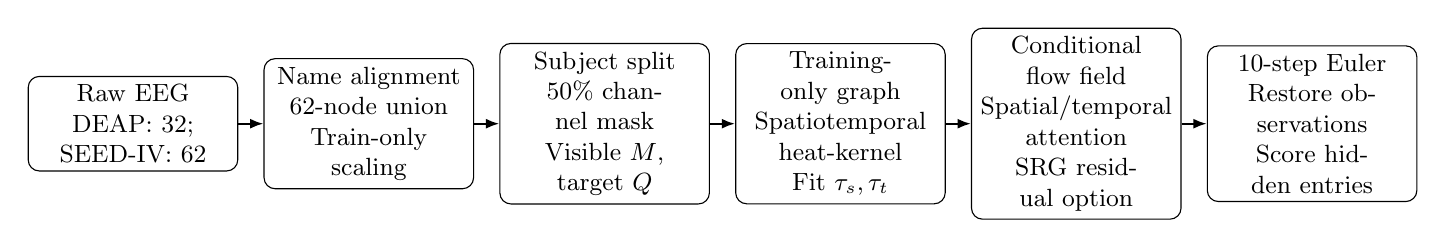
\begin{tikzpicture}[
  >=Latex,
  node distance=0.32cm,
  stage/.style={draw,rounded corners,align=center,
    minimum height=0.9cm,text width=2.45cm,inner sep=3pt,font=\small},
  arrow/.style={-{Latex[length=1.7mm]},thick}
]
\node[stage] (data) {Raw EEG\\DEAP: 32; SEED-IV: 62};
\node[stage,right=of data] (align) {Name alignment\\62-node union\\Train-only scaling};
\node[stage,right=of align] (mask) {Subject split\\50\% channel mask\\Visible $M$, target $Q$};
\node[stage,right=of mask] (prior) {Training-only graph\\Spatiotemporal heat-kernel\\Fit $\tau_s,\tau_t$};
\node[stage,right=of prior] (field) {Conditional flow field\\Spatial/temporal attention\\SRG residual option};
\node[stage,right=of field] (eval) {10-step Euler\\Restore observations\\Score hidden entries};
\draw[arrow] (data)--(align);
\draw[arrow] (align)--(mask);
\draw[arrow] (mask)--(prior);
\draw[arrow] (prior)--(field);
\draw[arrow] (field)--(eval);
\end{tikzpicture}%
}
\caption{Implemented EEG reconstruction workflow. Both models share
preprocessing, graph-informed initialization, and Euler inference;
SRG-flow adds residual guidance and step-dependent velocity calibration.}
\label{fig:pipeline}
\end{figure*}

\subsection{Data and Missing-Channel Task}

Let $X\in\mathbb{R}^{N\times R}$ be a complete window, $O$ indicate
genuinely recorded entries, $M$ the visible conditioning mask, and $Q$ the
artificially hidden evaluation mask. We require $M\odot Q=0$ and
$M+Q\leq O$. The model receives $X_{\mathrm{cond}}=M\odot X$ and is scored
only on $Q$; naturally absent samples and padded electrodes are excluded.
The primary evaluation hides half of available electrode traces.

DEAP-RAW uses 32 named EEG electrodes resampled to 200~Hz; raw SEED-IV
trials provide 62 channels \cite{koelstra2012deap,zheng2019emotionmeter}.
Canonicalized electrode names align both sources into a 62-node union.
Channels absent from a source are padded and marked unavailable, not treated
as observed zeros. Each source is standardized using training participants
only; predictions are returned to source units for evaluation.

The pilot selects 25 evenly spaced, non-overlapping 100-sample windows per
participant. Test participants are DEAP 03, 05, 11, 12, 22, and 26, and
SEED-IV 7, 10, and 15. Splits are participant-disjoint; joint training
samples the datasets equally. Training masks randomly retain 30--90\% of
available entries, with an additional 0.5 probability of dropping each
electrode. Point, block, and shared-stream masks are implemented but are not
evaluated in the reported real-data study.

\subsection{Graphs and GiFlow}

Spatial graphs are estimated from training windows only. For electrodes
$i,j$, edge distance is $d_{ij}=1-|r_{ij}|$, where $r_{ij}$ is their
signal correlation. The Gaussian weight
$w_{ij}=\exp[-(d_{ij}/\omega)^2]$ is thresholded at 0.1 and binarized;
$\omega$ is the standard deviation of off-diagonal distances. The joint
graph averages source edges only when both nodes are present. Time samples
form a line graph. Their Laplacians $L_s,L_t$ define a heat-kernel source:
\begin{equation}
X_0=\exp(-\tau_sL_s)(M\odot X)\exp(-\tau_tL_t).
\label{eq:source}
\end{equation}
Training-only optimization fits $\tau_s,\tau_t$ using signal-alignment and
spatial-smoothness loss
$\mathbb{E}[\|X-X_0\|_2^2+\alpha_\tau
\operatorname{tr}(X_0^\top L_sX_0)]$; the factors are then frozen.

For $t\sim\mathcal{U}(0,1)$, the linear flow path is
$X_t=(1-t)X_0+tX$, with target velocity $U_t=X-X_0$. The conditional
vector field receives $X_t$, visible signal, mask, and a time embedding.
Learned electrode embeddings and graph message passing support spatial
attention; temporal attention acts along samples, and alternating spatial
and temporal propagation fuses the representations. Training minimizes
masked velocity error on target entries plus an observed-value preservation
term, weighted by 0.1.

\subsection{SRG-Flow and Inference}

SRG-flow shares GiFlow's source, path, and base vector field $v_\theta$.
A residual module $r_\phi$ predicts the error direction
$U_t-\operatorname{stopgrad}(v_\theta)$; a time-conditioned module predicts
scale $\gamma_t$ and bias $\beta_t$. Its velocity is
\begin{equation}
v'_t=\gamma_t(v_\theta+\lambda_{\mathrm{res}}r_\phi)+\beta_t.
\end{equation}
Residual regression and an identity-calibration penalty
$(\gamma_t-1)^2+\beta_t^2$ are added to the training objective. This
adaptation uses neither a VAE nor a diffusion noise-prediction objective.

Both models use hidden dimension 64, four propagation layers, dropout 0.1,
batch size 32, Adam at $10^{-3}$, weight decay $5\times10^{-5}$, and a
maximum of 50 epochs with patience 8. The filtering stage runs for 20
epochs; validation NMSE selects the EMA checkpoint. No tau floor was used.
SRG-flow uses residual weight 1 and modulation penalty 0.01. All runs use
seed 0 on an NVIDIA RTX 4050. Inference uses 10 deterministic Euler steps,
restoring visible entries exactly after integration.

\section{Experiments and Results}

Six matched single-seed runs compare joint, DEAP-only, and SEED-IV-only
training for each learned model. Evaluation uses the same whole-channel
masks and held-out participants across variants. Joint-versus-individual
training changes both data and graph estimation, so it does not isolate
the effect of adding another training source. NMSE is the squared error on
$Q$ divided by reference energy on $Q$; PCC is computed over scored entries.
The macro score is the arithmetic mean of source-specific pooled NMSE.
The joint evaluation scores 240,000 hidden DEAP entries and 232,500 hidden
SEED-IV entries from the selected participant windows.

\begin{table*}[t]
\centering
\caption{NMSE/PCC on participant-held-out 50\% whole-channel loss. Lower
NMSE and higher PCC are better. Individual models are evaluated only on
their training source. All results use one seed.}
\label{tab:results}
\setlength{\tabcolsep}{3pt}
\begin{tabular}{lccc}
\toprule
Method & DEAP NMSE/PCC & SEED-IV NMSE/PCC & Macro NMSE\\
\midrule
Joint GiFlow & 0.5920/0.6261 & 0.6333/0.6313 & 0.6127\\
Joint SRG-flow & 0.5979/0.6219 & 0.6416/0.6248 & 0.6198\\
Joint KNN & 0.5931/0.6258 & 0.6113/0.6258 & 0.6022\\
Joint feature propagation & 0.6052/0.6167 & 0.6506/0.5913 & 0.6279\\
DEAP GiFlow & 0.6325/0.5942 & -- & --\\
DEAP SRG-flow & 0.8456/0.4247 & -- & --\\
SEED-IV GiFlow & -- & 0.7571/0.5351 & --\\
SEED-IV SRG-flow & -- & 0.7216/0.5409 & --\\
\bottomrule
\end{tabular}
\end{table*}

\begin{table}[t]
\centering
\caption{Fitted graph-filter factors and validation-selected epochs
(zero-based).}
\label{tab:taus}
\setlength{\tabcolsep}{3pt}
\begin{tabular}{llccc}
\toprule
Training & Model & Epoch & $\tau_s$ & $\tau_t$\\
\midrule
Joint & GiFlow & 2 & 0.0194 & 0.0381\\
Joint & SRG-flow & 2 & 0.0193 & 0.0469\\
DEAP & GiFlow & 40 & 2.5104 & 0.0528\\
DEAP & SRG-flow & 2 & 2.5685 & 0.0543\\
SEED-IV & GiFlow & 2 & 0.0476 & 0.0882\\
SEED-IV & SRG-flow & 3 & 0.0466 & 0.0792\\
\bottomrule
\end{tabular}
\end{table}

\begin{figure*}[t]
\centering
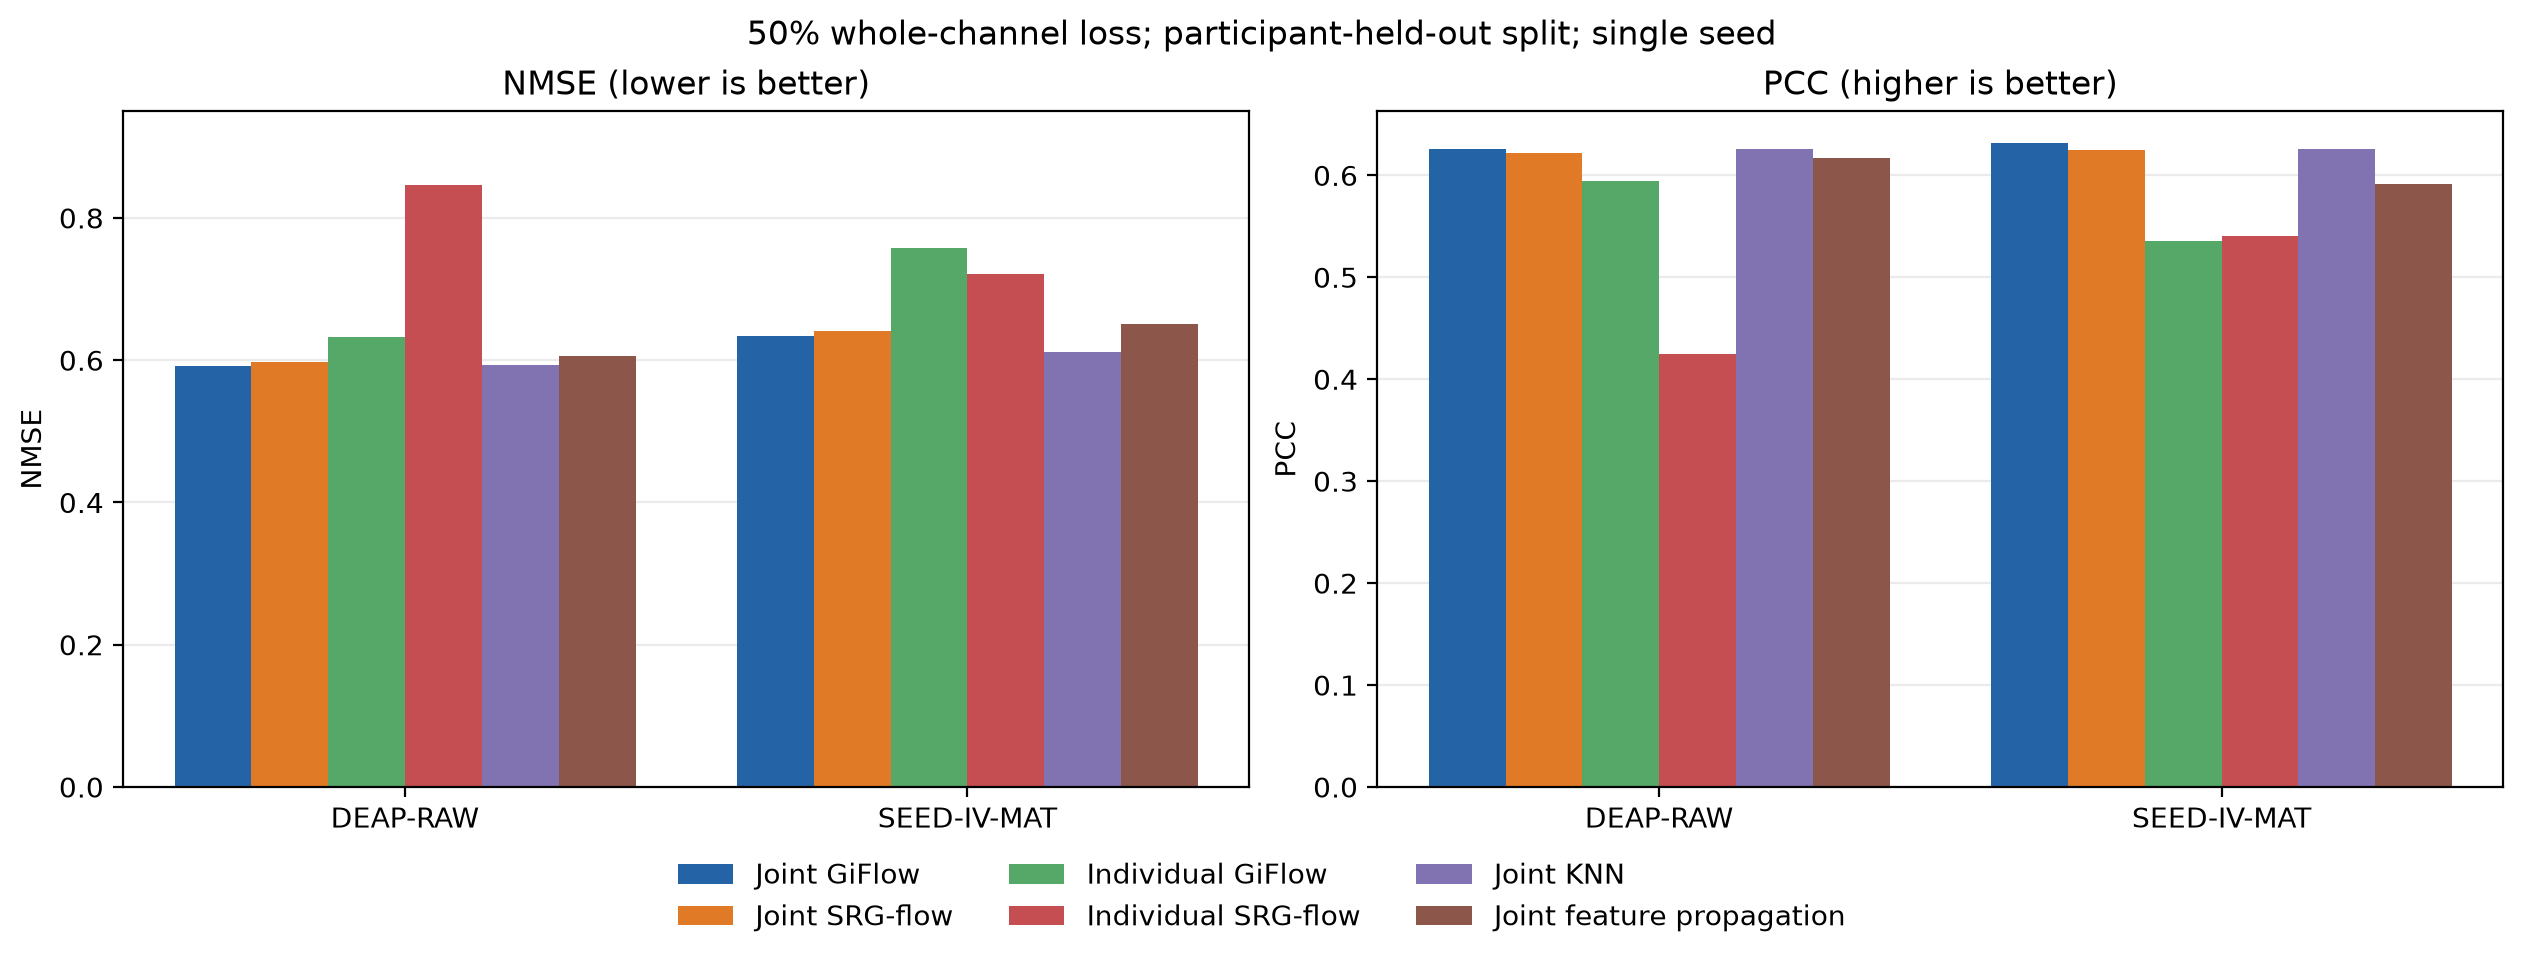
\includegraphics[width=0.96\textwidth]{figures/isbi2027_model_comparison.png}
\caption{NMSE and PCC for joint and source-specific models and interpolation
baselines on the matched seed-0, 50\% whole-channel, participant-held-out
evaluation. Bars show one split and do not represent between-seed
variability.}
\label{fig:comparison}
\end{figure*}

Joint GiFlow has the best learned-model NMSE on both sources, but its
advantage over KNN on DEAP is small (0.5920 versus 0.5931); KNN is better
on SEED-IV and has the lowest macro NMSE. SRG-flow is slightly worse than
GiFlow on both sources and does not improve the macro score. Joint training
is associated with lower NMSE than individual training for the corresponding
model in this split, but the simultaneous change in graph prevents a causal
interpretation. Source-specific KNN NMSE is 0.5964 on DEAP and 0.6097 on
SEED-IV, outperforming the corresponding individual learned models.
The fitted factors in Table~\ref{tab:taus} show substantially larger
spatial smoothing for the DEAP-only models than for the joint or SEED-IV
models; the pilot did not test a tau floor, so this is a diagnostic
observation rather than evidence that a floor would help.

Pooled results conceal participant variation. Equal-subject PCC/NMSE
($\mathrm{mean}\pm\mathrm{SD}$) for GiFlow is $0.124\pm0.421$ /
$0.691\pm0.477$ on DEAP and $0.618\pm0.131$ / $0.639\pm0.145$ on SEED-IV;
for SRG-flow it is $0.115\pm0.409$ / $0.754\pm0.531$ and
$0.610\pm0.137$ / $0.648\pm0.165$, respectively. The large DEAP dispersion
motivates participant-level reporting. The study is bounded to 25 windows
per participant and one seed; it does not test the other implemented masks,
tau floors, spectral or topographic error, or downstream emotion-task
utility. Different recording scales and acquisition protocols also limit
cross-source interpretation despite separate normalization.

\section{Conclusion}

In this single-seed, participant-held-out pilot, joint GiFlow outperforms
SRG-flow among learned methods, while KNN has the lowest macro NMSE.
Joint training is associated with lower error than individual training,
but also changes graph estimation. These results do not establish a
reliable advantage for learned flow reconstruction. Repeated seeds,
additional missingness patterns, controlled graph ablations, and
feature- or task-level evaluation are needed.

\section*{Compliance with Ethical Standards}
Authors: replace this note with the accurate ethics/compliance statement
for the datasets and applicable institutional requirements.

\section*{Acknowledgments}
Authors: add funding, conflict-of-interest, and any required AI-use
disclosure statements.

\bibliographystyle{IEEEbib}
\bibliography{isbi2027_references}

\end{document}
